%----------------------------------------------------------------------------
%----------------------------------------------------------------------------
%				    	SETUP
%----------------------------------------------------------------------------
%----------------------------------------------------------------------------

\documentclass[11pt]{article}

%----------------------------------------------------------------------------
%			  	   PACKAGES
%----------------------------------------------------------------------------

%%%%%%%%%%%%%%%%%%%%%%%
% 	  Packages
%%%%%%%%%%%%%%%%%%%%%%%

%% Fonts and Symbols
%% --------------------------
\usepackage{
			amsmath,			% math operators
			amssymb,			% math symbols
%			amsthm,				% theorem environment
			soul,				% strike through with \st{}
			xcolor,				% color!
%			xfrac,				% fancy fractions
}		

%% Graphics
%% --------------------
\usepackage{
			graphicx,			% allows insertion of images
			subfigure,			% allows subfigures (a), (b), etc.
}				
\graphicspath{ {graphics/} }	% (graphicx) relative path to graphics folder				

%% Tables
%% --------------------------
\usepackage{
			booktabs,			% better tables, discourages vertical rulings
			multicol,			% allow multi columns
%			tocloft,			% finer control over TOC; enabled below due to subfigure conflict
}
%\usepackage[subfigure]{tocloft}
%\addtocontents{toc}{\cftpagenumbersoff{subsubsection}} % turn off subsubsection page numbers in ToC

%% Layout Alteration
%% --------------------------
\usepackage{			
%			caption,			% line breaks in captions with \\
%			changepage,			% change margins for PARTS of pages with (adjustwidth)
			fancyhdr,			% see config in LAYOUT AND STYLING
			framed,				% nice boxes; used in Supervisor's Approval
%			fullpage,			% set full page margins
			geometry,			% change the margins for specific PAGES
%			lastpage,			% used with (fancyhdr)
			parskip,			% disable indents
%			pdflscape,			% ???
			rotating,			% sideways figures
}
\geometry{						% specify page size options for (geometry)
			a4paper, 			% paper size
			hmargin=1in,		% horizontal margins
			vmargin=1in,		% vertical margins
}	


%% Units
%% --------------------------
\usepackage{
			siunitx,			% has S (decimal align) column type
}
\sisetup{input-symbols = {()},  % do not treat "(" and ")" in any special way
		group-digits  = false, 	% no grouping of digits
%		 load-configurations = abbreviations,
%		 per-mode = symbol,
}

%% Misc
%% --------------------------
\usepackage{
			enumitem,			% better control of enumerations, descriptions, etc
}



%----------------------------------------------------------------------------
%		     MACROS AND COMMANDS
%----------------------------------------------------------------------------

% Defines a new command for the horizontal lines, change thickness here
\newcommand{\HRule}{\rule{\linewidth}{0.5mm}} 

% scientific notation  use \e
\providecommand{\e}[1]{\ensuremath{\times 10^{#1}}}

% override S column type with centered text column
\newcommand{\textcol}[1]{\multicolumn{1}{c}{#1}}

% easy unit spacing in math mode
\providecommand{\units}[1]{\;\text{#1}}

%----------------------------------------------------------------------------
%----------------------------------------------------------------------------
%				   DOCUMENT
%----------------------------------------------------------------------------
%----------------------------------------------------------------------------

\begin{document}

%----------------------------------------------------------------------------
%				    TITLE PAGE
%----------------------------------------------------------------------------

\begin{titlepage}

\center
 
% Header
\textsc{\LARGE University of Victoria}\\[1cm] 	% Name of your university/college
\textsc{\Large CENG 241}\\[0.5cm] 			% Major heading such as course name
\textsc{\large Digital Design I}\\[0.5cm] 		% Minor heading such as course title


% Lab Title
\HRule \\[0.4cm]
{ \huge \bfseries Lab 1 - Digital Instrumentation, Basic Digital Components and Circuits}\\[0.2cm] % Title of your document
\HRule \\[1.5cm]
 
 
%Lab Instructor Details
\begin{minipage}{0.7\textwidth}
\begin{flushleft} 

\large\emph{Instructor:} \\
Dr. Amirali \textsc{Baniasadi} \\
\vspace{12 pt}
\emph{Teaching Assistant:} \\
Grace \textsc{Hui}

\end{flushleft}
\end{minipage}
~
%% No content here, but it keeps the alignment of the instructor/TA
%% box correct.
%% Consider revising.
\begin{minipage}{0.1\textwidth}
\begin{flushright} \large
%Dr. Barbara \textsc{Sawicka} \\
\vspace{12 pt}
%\emph{Teaching Assistant:} \\
%Vahid \textsc{Moradi}
\end{flushright}
\end{minipage}\\[2cm]


% Lab members
\Large Yves \textsc{Senechal}
\large V00213837	\\
\Large Tyler \textsc{Stephen}
\large V00812021	\\
A01 - B03\\[1.5cm] 


% Date
{\large June 1, 2015}\\ % Date, change the \today to a set date if you want to be precise

% Logo
\begin{figure}[b]	 % put logo at bottom of the page
	\centering
	\includegraphics[scale=0.3]{UVic_logo}
\end{figure}

\end{titlepage}

%----------------------------------------------------------------------------
%				    BODY
%----------------------------------------------------------------------------

\section{Introduction}

This lab serves as an introduction to basic digital components and circuits. The following is a list of items explored throughout this lab:

\begin{itemize}

	 \item voltage regulator 
 	 \item power supply
	 \item oscilloscope
	 \item pulse generator
	 \item digital multimeter
	 \item SPDT switch
	 \item push button debouncer
	 \item and various electrical components.
	  
\end{itemize}

\section{Voltage Regulators}
\begin{table}[h]
	\centering
	\begin{tabular}{ @{} S S S S S S @{} }
		\toprule
		\textcol{$V_{in}$ (V)} &
			\textcol{$V_{out}$ (V)} &
			\textcol{$I_{in}$ (mA)} &
			\textcol{$I_{out}$ (mA)} &
			\textcol{$P$ (mW)} &
			\textcol{$T$ (\si{\celsius})} \\
		\midrule
		0.0	& 2e-5		& 2e-4		& 2e-4		& N/A & 22.9 \\
		1.0	& 1.5e-5	& 2e-4		& 2e-4		& N/A & 22.9 \\
		2.0	& 4.3e-4	& 6e-4		& 6e-4		& N/A & 23.3 \\
		3.0	& 1.5913	& 1.599		& 1.599		& 2.25 & 23.0 \\
		4.0	& 2.5057	& 2.5143	& 2.5143	& 3.76 & 23.2 \\
		5.0	& 3.662		& 3.6758	& 3.6758	& 4.92 & 23.4 \\
		6.0	& 4.689		& 4.7083	& 4.7083	& 6.17 & 23.8 \\
		7.0	& 4.992		& 5.0129	& 5.0129	& 10.1 & 24.1 \\
		8.0	& 4.904		& 4.9252	& 4.9252	& 15.2 & 24.8 \\
		9.0	& 4.845		& 4.8655	& 4.8655	& 20.2 & 25.7 \\
		10.0& 4.815		& 5.053		& 5.053		& 26.2 & 25.8 \\
		11.0& 4.777		& 5.050		& 5.050		& 31.4 & 26.3 \\
		12.0& 4.759		& 5.0217	& 5.0217	& 36.4 & 27.2 \\
		\bottomrule
	\end{tabular}
	\caption{Voltage, current and temperature response of LM7805 5V regulator}
	\label{table:regulator}
\end{table}

The voltage regulator regulated the output voltage to \SI{5.0 +- 0.3}{\volt} for input voltages between \SI{6.0}{\volt} and \SI{12.0}{\volt}. As we can see in Table \ref{table:regulator}, when the power supply was set to below \SI{3.0}{\volt} only stray voltages and currents were present; the voltage regulator blocked insufficient voltages and currents. As the regulator worked to regulate the voltage its power consumption increased, which was evident by the heat dissipated.   

Next, the output of the voltage regulator was shorted to ground. Initially, the power supply was set to \SI{8}{V} and \SI{200}{mA}; however, the power supply limited the voltage and current to \SI{2.7}{\volt} and \SI{130}{mA} due to its short circuit protection. The regulator controlled the output to \SI{64.47}{\milli\volt} and \SI{136}{\milli\ampere}, while increasing its operating temperature from room temperature to \SI{44.8}{\celsius}.

\section{Signal damping}

Figure \ref{fig:damping} displays\footnote{Oscilloscope screen captures are included after the conclusion.} examples of over-damped, under-damped, and critically damped waveforms. Properly tuned oscilloscope probes will display a critically damped waveform when tested, and they should be tested prior to every use.

Figure \ref{fig:rise_fall} illustrates the rise and fall time of critically tuned probes.  The rise and fall times were both calculated to be \SI{1.00 +- 0.04}{\micro\second}.

\section{LEDs and Inverters}

The LED illuminated in the absence of the signal voltage, while it extinguished at the presence of it. Since the signal voltage was inverted, the LED was connected to the source voltage and the circuit was completed only at the absence of a signal.

\begin{figure}[h]
	\centering
	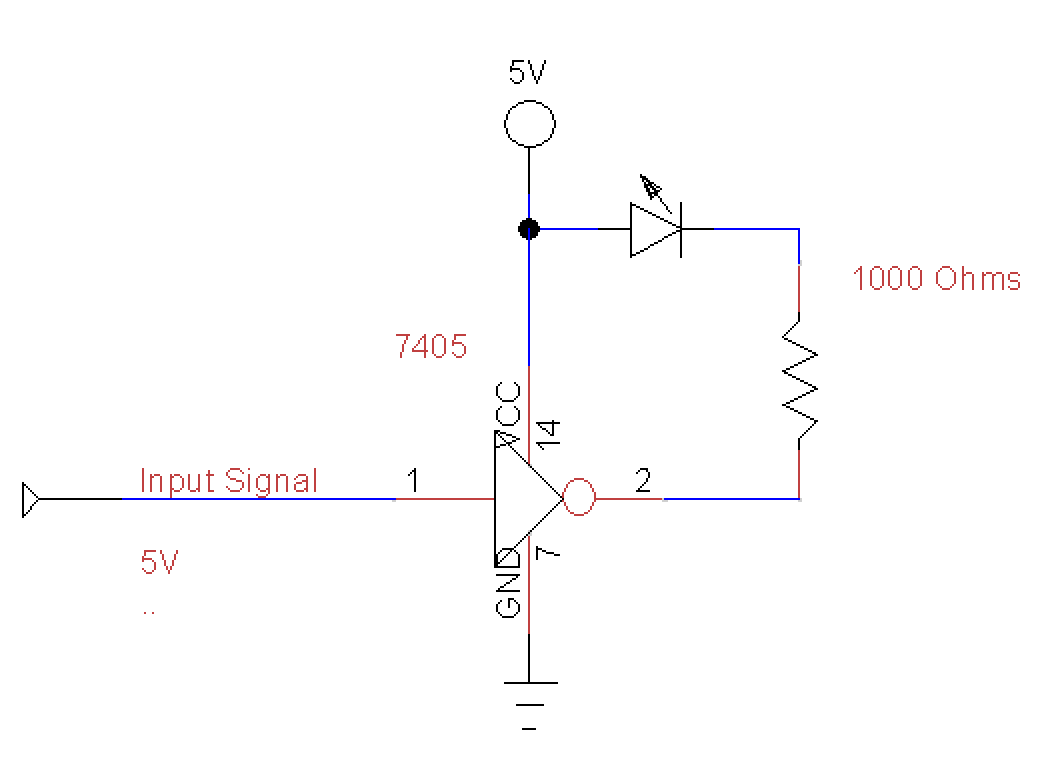
\includegraphics[scale=0.6, draft=false]{inverter}
	\caption{Controlling an LED with a LS7405 inverter.}
	\label{fig:inverter}
\end{figure}

The 7405 inverter features open collector outputs, while the 7404 does not. The 7404 inverter connects internally the $V_{cc}$ to the output by way of an internal transistor through a \SI{130}{\ohm} resistor. Our circuit configuration would then place a parallel run with the LED and external \SI{1}{\kilo\ohm} resistor. Since the current will chose the path of least resistance, there would not be enough current to power the LED. 

\section{Push button debouncing}

Actually existing switches are analogue devices, in the sense that the transition between open and closed states is not instantaneous. A button ``bounces'' when it permits a voltage level which is in between the high and low voltage logic levels. Two NAND gates can be combined into an SR flip-flop, which can be used to debounce buttons. Figure \ref{fig:debounce} displays the debounced and non-debounced waveforms from activating the push button. The non-debounced signal switches between high and low levels while the voltage is in an intermediate value. In contrast, the debounced signal transitions to the low level and does not switch back to high. The debounced signal allows the signal to be processed faster because there is no ``settling'' time.

A debouncer can be implemented using NOR gates, figure \ref{fig:nor_gates} illustrates such a circuit. 

\begin{figure}[h]
	\centering
	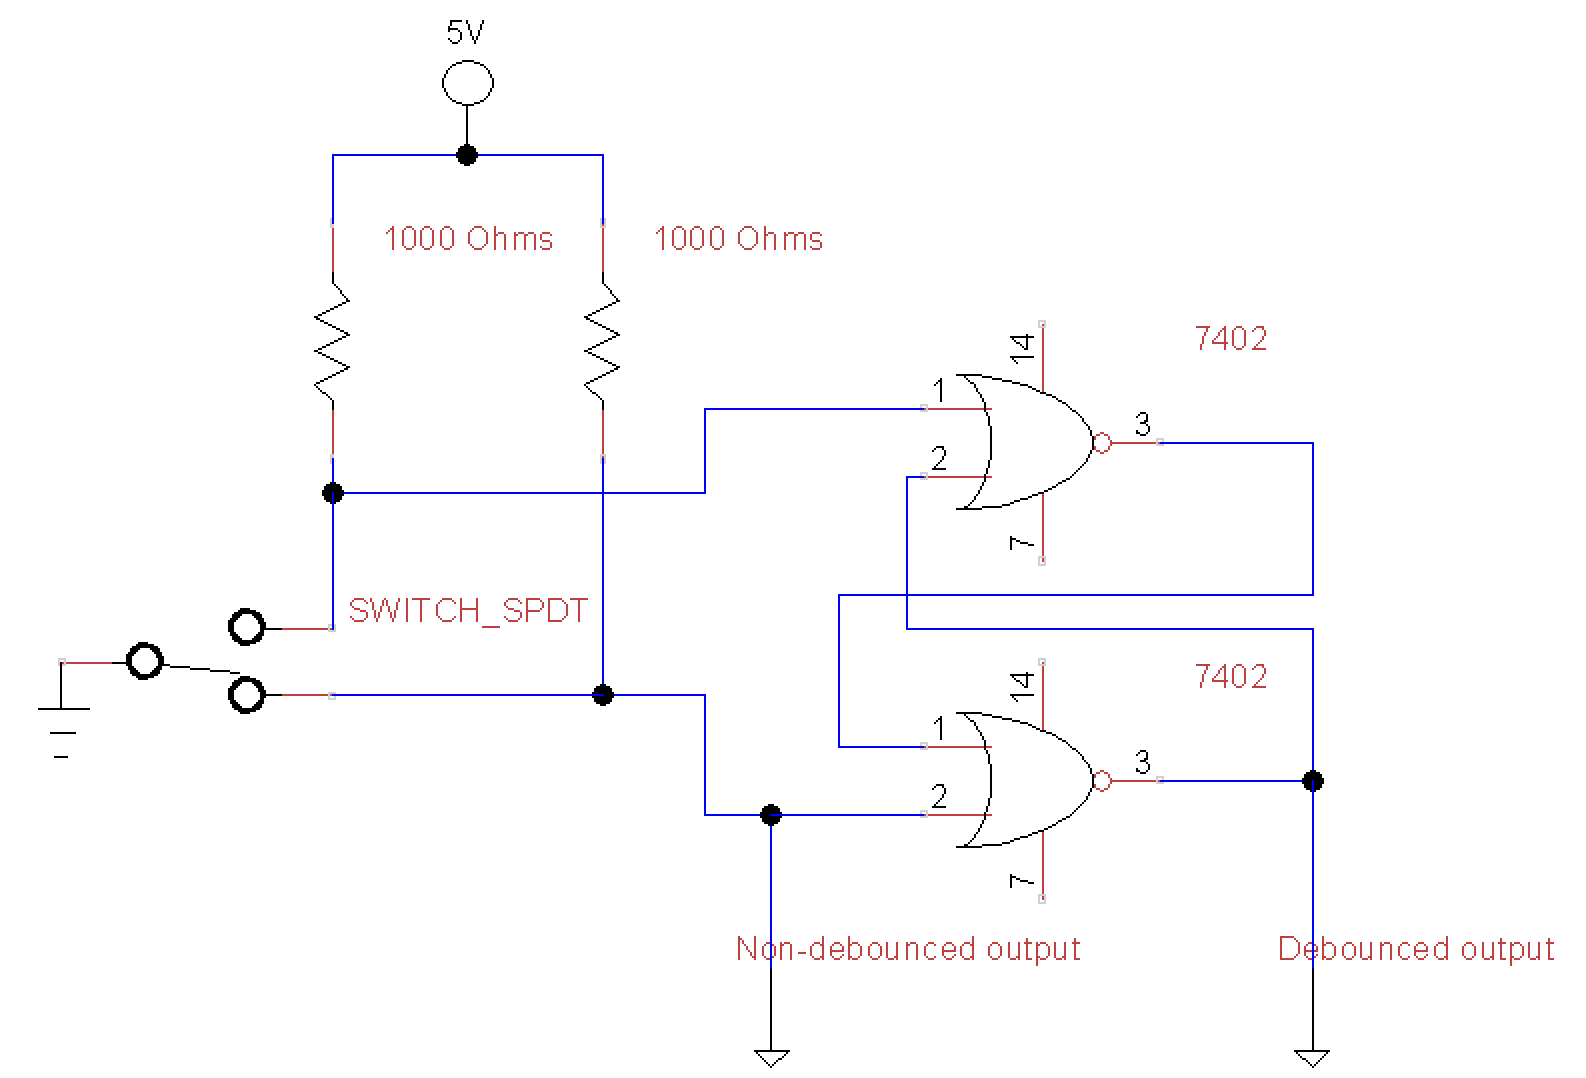
\includegraphics[scale=0.5, draft=false]{nor_gates}
	\caption{An SPDT debouncer constructed from NOR gates. For clarity, $V_{cc}$ (pin 14) and ground (pin 7) are not connected in the schematic.}
	\label{fig:nor_gates}
\end{figure}

\section{Conclusion}

While being introductory, the circuits explored in this lab performed as expected. The voltage regulator dissipates heat fast under extreme circumstances, but its temperature only increases gradually when used under normal conditions. Also, circuits can be analyzed cleanly with properly tuned oscilloscope probes, an status circuit with LED, and a debouncer. These items help to expedite and facilitate troubleshooting.

\section*{Oscilloscope screen captures}

\begin{sidewaysfigure}[h]
	\centering
	\subfigure[Over damping]
	{
		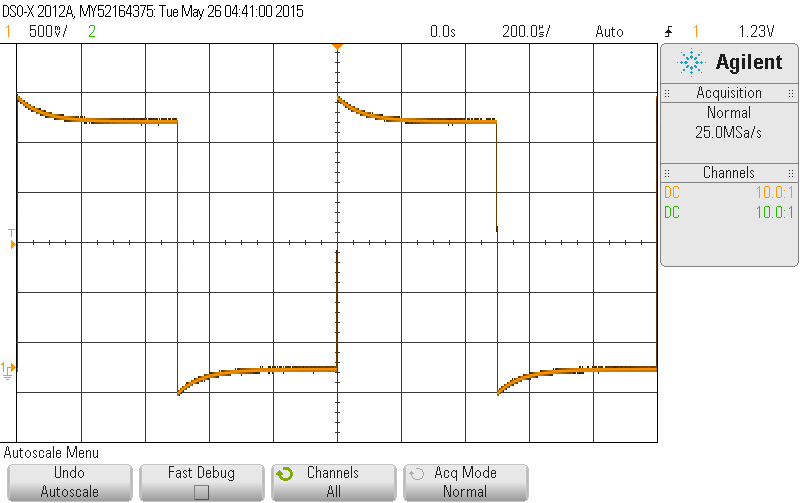
\includegraphics[width=0.475\textwidth, draft=false]{overdamped}
	}
	\subfigure[Under damping]
	{
		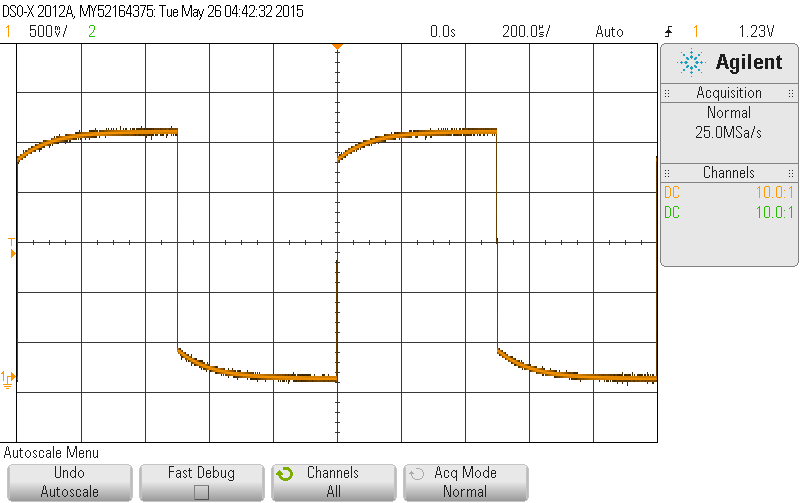
\includegraphics[width=0.475\textwidth, draft=false]{underdamped}
	}
	\subfigure[Critical damping]
	{
		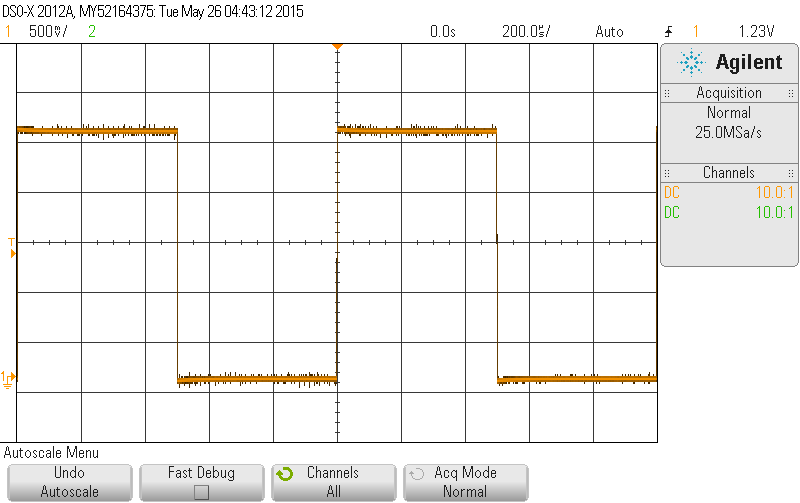
\includegraphics[width=0.475\textwidth, draft=false]{critdamped}
	}
	\caption{Waveforms representative of different levels of damping for a square wave}
	\label{fig:damping}
\end{sidewaysfigure}

\begin{figure}[h]
	\centering
	\subfigure[Rise time]
	{
		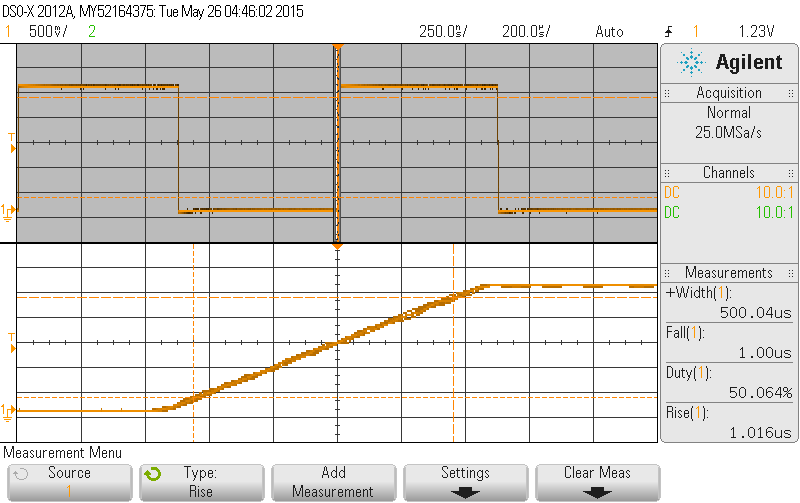
\includegraphics[width=0.95\textwidth, draft=false]{risetime}
	}
	\subfigure[Fall time]
	{
		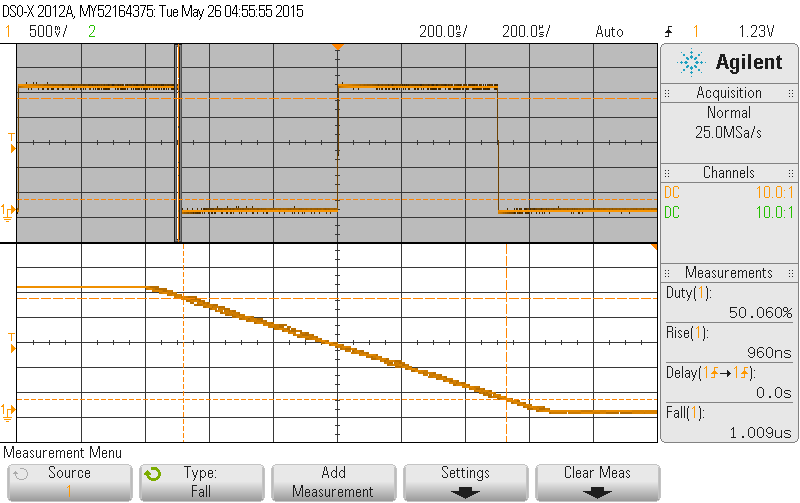
\includegraphics[width=0.95\textwidth, draft=false]{falltime}
	}
	\caption{Opposite edges of a critically damped square wave}
	\label{fig:rise_fall}
\end{figure}

\begin{figure}[h]
	\centering
	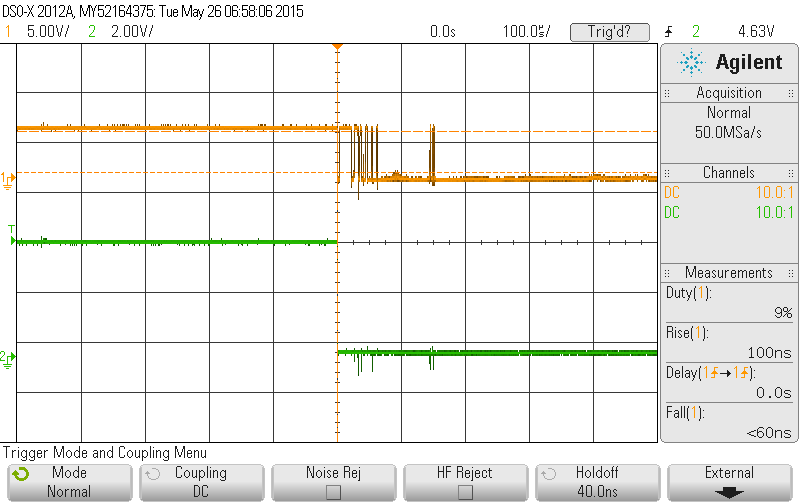
\includegraphics[width=0.95\textwidth, draft=false]{debounce}
	\caption{Waveforms of non-debounced (top) and debounced (bottom) SPDT presses}
	\label{fig:debounce}
\end{figure}

\end{document}